\chapter{Análisis y tratamiento de datos}
\label{chap:ia}

Para implementar un sistema de Inteligencia Artificial, en adelante \textit{IA}, que clasifique un conjunto de datos, necesitaremos obtener mucha información para \textit{alimentarla}. Estos datos normalmente en bruto contienen información redundante, valores atípicos, campos nulos\dots~ todo esto haría que nuestra \textit{IA} se viese afectada negativamente, para ello necesitaremos tratar correctamente los datos.

En la última parte del capítulo se seguirá el proceso de selección de los algoritmos más plausibles, así como su ajuste para refinar progresivamente los modelos elaborados.

En el Capítulo \ref{chap:resultados}, se mostrarán y analizarán los resultados obtenidos después de realizar el procedimiento mencionado en este capítulo.

\section{Tratamiento de los datos}

La mayoría de los de algoritmos de aprendizaje presentan varias necesidades previas a la hora de trabajar con un conjunto de datos. Por ello, se necesita procesar la información y formatearla correctamente para los entrenamientos. 
En esta sección se abordarán las técnicas empleadas para solventar dicho problema.

\subsection{Variables de texto}

La mayoría de los algoritmos de aprendizaje mejor con números que con etiquetas. Para que nuestros datos se adecuen a estas circunstancias debemos manipularlos correctamente.


Nuestro conjunto de datos solo presenta una variable de texto que es la de usuario, la cual hace referencia al dueño del evento. Para formatear estos valores a números, se ha usado una función de la librería de \textit{Sklearn}, la cual asigna un único valor a cada etiqueta.
 \subsection{Variables categóricas}
 Estas variables representa un conjunto de datos, es decir, cada valor representa una categoría.
 
En nuestro caso el dato dirección es una variable categórica, en la cual cada valor representa una dirección única. Sino formateamos este valor, el algoritmo entenderá que los valores más próximos están más relacionados.
Para solucionar este problema hemos usado una función de la librería de \textit{Sklearn}, la cual genera una columna por cada valor posible y le asigna el valor cero o uno en función del valor de la columna original~[Tabla~\ref{tab:categorical_feature}].

\begin{table}[H]
    \centering
    \begin{tabular}{ c || c c c }
\toprule
\textbf{Columna Original} & \multicolumn{3}{c}{\textbf{Columna Transformada}} \\
\midrule
direction &  direction\_4 &  direction\_8 &  direction\_16 \\
\midrule
8  &             0 &            1 &             0 \\
4  &             1 &            0 &             0 \\
16 &             0 &            0 &             1 \\
\bottomrule
\end{tabular}
    \caption{Corrección de la variable categórica}
    \label{tab:categorical_feature}
\end{table}

\subsection{Valores Nulos}

La mayoría de los algoritmos de aprendizaje no pueden trabajar con valores nulos, por lo tanto, necesitamos tratar nuestros datos para detectarlos y procesarlos correctamente. 
Para realizar este paso se contemplaron las siguientes opciones:

\begin{enumerate}
    \item Eliminar la fila que los contiene.
    \item Eliminar la columna que los contiene.
    \item Rellenar a cero dichos valores.
    \item Rellenar los valores con la mediana.
\end{enumerate}

De las opciones mencionas se eligió la última ya que es menos agresiva a la hora de modificar los datos. La librería de \textit{Sklearn} proporciona un método que nos ayuda con este proceso, y asigna a los valores nulos el valor que hemos escogido, en nuestro caso la mediana.

\subsection{Transformación de las características}

Para encontrar nuevas relaciones entre las características y las clases se ha utilizado el método de \textit{polynomial feature} de la librería \textit{Sklearn}.

En el ejemplo de la Figura~\ref{fig:polynomial} la imagen de la izquierda representa un problema linealmente no separable. Pero si elevamos al cuadrado la características $x_1$ los datos pasan a ser linealmente separables.

\begin{figure}[h]
    \centering
    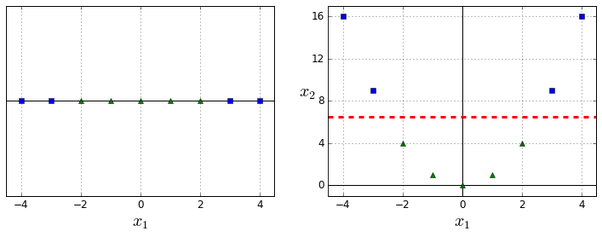
\includegraphics[width=0.8\textwidth, keepaspectratio]{imaxes/polinomial.png}
    \caption{Ejemplo de Polynomial Feature}
    \label{fig:polynomial}
\end{figure}

En este proyecto se utilizo esta técnica para generar características de segundo grado, es decir, si tenemos las características $[a, b]$, el segundo grado sería $[1, a, b, a^2, ab, b^2]$.

\subsection{Estandarizar los datos}
La mayor parte de los algoritmos de aprendizaje disminuyen su rendimiento cuando los valores de las variables se mueven en un rango muy amplio. Dentro de las características de los eventos existen varias variables con esta problemática, como es el caso de \textit{duración}. Esta variable tiene un valor medio de 122 \textit{ms} mientras que su rango de valores es~[13, 1654]~[Tabla~\ref{tab:scaler_example}].

\begin{table}[H]
    \centering
    \begin{tabular}{lrrrrrrrr}
        \toprule
        {} &   count &        mean &        std &   min &   25\% &    50\% &    75\% &     max \\
        \midrule
        duration &  3436.0 &  122.40 &  72.48 &  13.0 &  83.0 &  104.0 &  146.0 &  1654.0 \\
        \bottomrule
    \end{tabular}
    \caption{Estadísticas de la característica duración}
    \label{tab:scaler_example}
 \end{table}
 
 Para realizar esta tarea se hace uso de la librería \textit{Sklearn}, la función utilizada realiza el siguiente proceso:
\begin{itemize}
\item Resta el valor medio, lo cual hace que los valores cerca de la media tiendan a cero.
\item Divide el valor por el rango intercuartílico~\footnote{Diferencia entre el tercer y el primer cuartil}. Se usan los cuartiles como valor de división porque hace que sea menos propenso a los valores atípicos
\end{itemize}

\section{Selección de algoritmos}

Para realizar las pruebas iniciales se han seleccionado los siguientes algoritmos:

\begin{itemize}
    \item \textbf{LogisticRegression (LR)}~(Véase Sección~[\ref{sec:logistic_regresion})
    
    \item \textbf{RandomForest (RF)}~(Véase Sección~\ref{sec:random_forest})
    
    \item \textbf{DecisionTree (DT)}~(Véase Sección~\ref{sec:decision_tree})
    
    \item \textbf{Perceptrón Multicapa (MLP)}~(Véase Sección~\ref{sec:mlp})
    
    \item \textbf{K-Nearest Neighbors (kNN)}~(Véase Sección~\ref{sec:kn})
    
    \item \textbf{Máquinas de soporte vectorial (SVM)}~(Véase Sección~\ref{sec:svm})
\end{itemize}

El primer paso consiste en realizar una prueba para tener un punto de inicio sobre el cuál comparar los resultados, y de esta manera comprobar analíticamente si las técnicas aplicadas a lo largo del capítulo han servido para mejorar la clasificación.

Analizando los resultados de la Tabla~\ref{table:clf_alg} en general todos los algoritmos obtienen unos valores similares en las columnas de \textit{Recall}, \textit{Precision} y \textit{F1 Score}, con una desviación del ±5\%. Si comparamos los resultados de los algoritmos individualmente podemos obtener las siguientes conclusiones:

\begin{itemize}
    \item \textbf{\textit{RF}}: Los resultados obtenidos por este algoritmo en la columna de \textit{precision} son los más altos exceptuando el evento de \textit{tap}. Los tiempos de entrenamiento (\textit{Fit Time}) están muy por debajo del resto de algoritmos.

    \item \textbf{\textit{DT}}: Los valores de las columnas de \textit{Recall}, \textit{Precision} y \textit{F1 Score} se mantienen en un rango de valores pequeño. 

    \item \textbf{\textit{LR}}: Los valores obtenidos en la columna \textit{precision} son los segundos más altos excepto en \textit{tap} donde es el más alto y, al igual que \textit{RF} el tiempo de entrenamiento suele ser bajo.
    
    \item \textbf{\textit{MLP}}: Los tiempos de predicción (\textit{Score Time}) obtenidos son los más bajos en todos los eventos.

    \item \textbf{\textit{SVM}}: Su desviación es la más alta y, por lo tanto, optimizando sus parámetros podría reducirse esta desviación y mejorando los resultados.

    \item \textbf{\textit{kNN}}: Este algoritmo obtuvo el rendimiento más bajo tanto en \textit{precision} como en \textit{Fit Time}.
\end{itemize}

Para reducir el tiempo de procesamiento y optimizar la búsqueda se ha decidido los siguientes algoritmos:
\begin{itemize}
    \item (\textit{DT}) debido a que \textit{RF} obtiene mejores resultados y al ser este un conjunto de \textit{DT} es redundante entrenar dos algoritmos de características similares. 
    \item \textit{KN} porque sus valores son lo que han obtenido el rendimiento más bajo.
\end{itemize}



\begin{table}[!h]
\centering
\begin{tabular}{ c l c c c c c }
\toprule
Evento & Alg. &  Recall & Precision & F1 Score & \thead{Fit \\ Time (s)} & \thead{Score \\ Time (s)} \\
\midrule
\multirow{6}{*}{\rotatebox[origin=c]{90}{motion}} &  \textit{DT} &  71.01\% (±0.122) &  71.96\% (±0.10 8) &  71.11\% (±0.110) &  0.072 &  0.121 \\
& \textit{kNN} &  70.85\% (±0.122) &  70.48\% (±0.108) &  70.29\% (±0.110) &  0.225 &  0.125 \\
& \textit{LR} &  71.22\% (±0.130) &  73.14\% (±0.112) &  71.76\% (±0.115) &  0.088 &  0.182 \\
& \textit{MLP} &  71.66\% (±0.120) &  71.48\% (±0.107) &  71.22\% (±0.107) &  0.269 &  0.094 \\
& \textit{RF} &  71.09\% (±0.135) &  76.33\% (±0.104) &  73.33\% (±0.118) &  0.054 &  0.324 \\
& \textit{SVM} &  69.01\% (±0.139) &  70.82\% (±0.123) &  69.08\% (±0.118) &  0.193 &  0.118 \\
\midrule
\multirow{6}{*}{\rotatebox[origin=c]{90}{multitouch}}  &  \textit{DT} &  71.45\% (±0.126) &  72.55\% (±0.110) &  71.58\% (±0.112) &  0.073 &  0.145 \\
 & \textit{kNN} &  70.98\% (±0.120) &  70.82\% (±0.107) &  70.51\% (±0.108) &  0.251 &  0.103 \\
 & \textit{LR} &  71.70\% (±0.131) &  74.40\% (±0.108) &  72.55\% (±0.113) &  0.044 &  0.246 \\
 & \textit{MLP} &  71.61\% (±0.121) &  71.75\% (±0.108) &  71.30\% (±0.108) &  0.147 &  0.105 \\
 & \textit{RF} &  75.95\% (±0.120) &  77.86\% (±0.097) &  76.52\% (±0.104) &  0.048 &  0.326 \\
 & \textit{SVM} &  69.74\% (±0.138) &  71.00\% (±0.119) &  69.53\% (±0.115) &  0.206 &  0.122 \\
\midrule
\multirow{6}{*}{\rotatebox[origin=c]{90}{orientation}} &  \textit{DT}  &  71.86\% (±0.121) &  72.82\% (±0.106) &  71.95\% (±0.108) &  0.071 &  0.128 \\
 & \textit{kNN}&  71.37\% (±0.120) &  71.01\% (±0.106) &  70.81\% (±0.107) &  0.233 &  0.118 \\
 & \textit{LR}&  72.25\% (±0.130) &  74.53\% (±0.107) &  72.95\% (±0.112) &  0.072 &  0.199 \\
 & \textit{MLP}&  72.13\% (±0.119) &  72.02\% (±0.105) &  71.72\% (±0.106) &  0.220 &  0.097 \\
 & \textit{RF}&  75.41\% (±0.110) &  79.54\% (±0.086) &  77.14\% (±0.096) &  0.053 &  0.325 \\
 &\textit{SVM} &  69.51\% (±0.138) &  71.38\% (±0.119) &  69.61\% (±0.115) &  0.196 &  0.119 \\
\midrule
\multirow{6}{*}{\rotatebox[origin=c]{90}{pan}} &   \textit{DT} &  70.96\% (±0.122) &  71.71\% (±0.110) &  70.97\% (±0.110) &  0.069 &  0.115 \\
& \textit{kNN}&  70.65\% (±0.129) &  70.06\% (±0.111) &  69.93\% (±0.113) &  0.218 &  0.128 \\
& \textit{LR}&  70.59\% (±0.129) &  72.38\% (±0.113) &  71.05\% (±0.115) &  0.084 &  0.168 \\
& \textit{MLP}&  71.19\% (±0.122) &  71.11\% (±0.108) &  70.75\% (±0.110) &  0.271 &  0.090 \\
& \textit{RF}&  70.29\% (±0.133) &  75.78\% (±0.110) &  72.60\% (±0.121) &  0.053 &  0.324 \\
&\textit{SVM} &  67.57\% (±0.162) &  71.14\% (±0.125) &  67.91\% (±0.137) &  0.188 &  0.115 \\
\midrule
\multirow{6}{*}{\rotatebox[origin=c]{90}{swipe}} &  \textit{DT}  &  72.07\% (±0.125) &  73.09\% (±0.109) &  72.17\% (±0.111) &  0.070 &  0.136 \\
&\textit{kNN}&  71.42\% (±0.120) &  71.18\% (±0.107) &  70.92\% (±0.108) &  0.242 &  0.111 \\
&\textit{LR}&  73.25\% (±0.132) &  75.39\% (±0.106) &  73.87\% (±0.113) &  0.044 &  0.220 \\
&\textit{MLP}&  72.20\% (±0.121) &  72.13\% (±0.106) &  71.80\% (±0.108) &  0.158 &  0.101 \\
&\textit{RF}&  77.98\% (±0.104) &  80.90\% (±0.091) &  79.13\% (±0.094) &  0.049 &  0.326 \\
&\textit{SVM}&  69.97\% (±0.137) &  71.44\% (±0.120) &  69.88\% (±0.115) &  0.201 &  0.120 \\
\midrule
\multirow{6}{*}{\rotatebox[origin=c]{90}{tap}} &   \textit{DT} &  70.55\% (±0.125) &  72.10\% (±0.111) &  70.92\% (±0.112) &  0.078 &  0.156 \\
& \textit{kNN} &  71.17\% (±0.120) &  71.11\% (±0.106) &  70.76\% (±0.108) &  0.261 &  0.098 \\
& \textit{LR} &  70.15\% (±0.125) &  74.98\% (±0.108) &  72.15\% (±0.114) &  0.046 &  0.280 \\
& \textit{MLP} &  71.03\% (±0.119) &  71.74\% (±0.109) &  71.03\% (±0.108) &  0.140 &  0.110 \\
& \textit{RF}  &  68.49\% (±0.072) &  73.82\% (±0.082) &  70.98\% (±0.075) &  0.048 &  0.327 \\
& \textit{SVM} &  70.72\% (±0.128) &  70.15\% (±0.111) &  70.00\% (±0.112) &  0.212 &  0.125 \\
\bottomrule
\end{tabular}

\caption{Resultados de la primera ejecución}
\label{table:clf_alg}
\end{table}

\newpage

\section{Selección de hiperparámetros }

En esta sección se verá cómo se han configurado los algoritmos. Dicha configuración se materializa a través de los hiperparámetros. Estos son valores que se establecen antes del entrenamiento del algoritmo y que deciden en parte como van a funcionar dichos algoritmos, permitiendo que se ajusten mejor al modelo.

Para buscar estos hiperparámetros  Se suelen utilizar dos técnicas:
\begin{itemize}
    \item \textbf{\textit{Grid Seach}}: Es un busca exhaustiva de los mejores parámetros sobre una combinación dada.
    \item \textbf{\textit{Random Search}}: Es un búsqueda aleatoria sobre una combinación de parámetros dada.
\end{itemize}

Para este proyecto se ha usado la técnica de \textit{Grid Search} como la idónea debido a publicaciones~\cite{bergstra2012random} sobre el rendimiento de ambas técnicas. 

Para analizar los resultados y obtener un valor los más aproximado posible se han seguido los siguientes pasos:
\begin{enumerate}
    \item Se han ordenado los resultados en orden descendente y se han seleccionado los cinco mejores valores de cada algoritmo.
    \item Se han calculado las puntuaciones medias de esos valores y su desviación, con el fin de obtener unos tiempos y puntuaciones medios [Tabla \ref{tab:mean_hyper_values}] para los mejores hiperparámetros.
    \item Se han calculado también los valores más comunes para obtener los mejores hiperparámetros  [Tabla \ref{tab:searched_hyper}].
\end{enumerate}


\begin{table}[!h]
    \centering
\begin{tabular}{c l c c c }
\toprule
Evento & Alg. &   Precision & Fit Time (s) & Score Time (s) \\
\midrule
\multirow{4}{*}{\rotatebox[origin=c]{90}{motion} }
&  \textit{LR}    &   63.23\% (± 0.047) & 1.1629 (± 0.047)  &   0.0268 (± 0.047)\\
& \textit{MLP}   &   65.79\% (± 0.080) & 10.4182 (± 0.080) &   0.0923 (± 0.080)\\
& \textit{RF}    &   68.42\% (± 0.060) & 0.3167 (± 0.060)  &   0.0160 (± 0.060)\\
& \textit{SVM}   &   65.64\% (± 0.132) & 0.1740 (± 0.132)  &   0.0762 (± 0.132)\\
\midrule

\multirow{4}{*}{\rotatebox[origin=c]{90}{multitouch} }
& \textit{LR}   &    76.98\% (± 0.128) & 0.0346 (± 0.128) &  0.0164 (± 0.128)\\
& \textit{MLP}  &    80.99\% (± 0.030) & 0.6049 (± 0.030) &  0.0218 (± 0.030)\\
& \textit{RF}   &    86.93\% (± 0.089) & 0.0811 (± 0.089) &  0.0091 (± 0.089)\\
& \textit{SVM}  &   100.00\% (± 0.000) & 0.0059 (± 0.000) &  0.0043 (± 0.000) \\
\midrule

\multirow{4}{*}{\rotatebox[origin=c]{90}{orienntation} }
& \textit{LR}   &    70.09\% (± 0.069) & 12.5253 (± 0.069) &  0.0248 (± 0.069)\\
& \textit{MLP}  &    66.72\% (± 0.033) & 28.8783 (± 0.033) &  0.1177 (± 0.033)\\
& \textit{RF}   &   77.28\% (± 0.048) & 0.1783 (± 0.048) &   0.0133 (± 0.048)\\
& \textit{SVM}  &   90.43\% (± 0.152) & 0.1458 (± 0.152) &   0.0746 (± 0.152)\\
\midrule

\multirow{4}{*}{\rotatebox[origin=c]{90}{pan} }
& \textit{LR}   & 67.48\% (± 0.148) & 0.1268 (± 0.148) &     0.0103 (± 0.148)\\
& \textit{MLP}  & 77.65\% (± 0.089) & 1.1181 (± 0.089) &     0.0334 (± 0.089)\\
& \textit{RF}   & 80.99\% (± 0.094) & 0.1343 (± 0.094) &     0.0122 (± 0.094)\\
& \textit{SVM}  & 78.96\% (± 0.099) & 0.0067 (± 0.099) &     0.0045 (± 0.099)\\
\midrule

\multirow{4}{*}{\rotatebox[origin=c]{90}{swipe} }
& \textit{LR}   &  84.67\% (± 0.043) & 0.5641 (± 0.043) &    0.0241 (± 0.043)\\
& \textit{MLP}  &  81.14\% (± 0.044) & 0.7857 (± 0.044) &    0.0822 (± 0.044)\\
& \textit{RF}   &  85.56\% (± 0.045) & 0.1575 (± 0.045) &    0.0130 (± 0.045)\\
& \textit{SVM}  &  94.07\% (± 0.066) & 0.0847 (± 0.066) &    0.0383 (± 0.066)\\
\midrule
\multirow{4}{*}{\rotatebox[origin=c]{90}{tap}}
& \textit{LR}    & 70.54\% (± 0.080) & 0.1695 (± 0.080) &     0.0149 (± 0.080)\\
& \textit{MLP}   & 75.42\% (± 0.090) & 7.6387 (± 0.090) &     0.1006 (± 0.090)\\
& \textit{RF}    & 75.52\% (± 0.092) & 0.1926 (± 0.092) &     0.0149 (± 0.092)\\
& \textit{SVM}   & 85.90\% (± 0.100) & 0.0768 (± 0.100) &     0.0278 (± 0.100)\\
\bottomrule
\end{tabular}
\caption{Resultados medios con los mejores hiperparámetros }
    \label{tab:mean_hyper_values}
\end{table}


\begin{table}[H]
    \centering
    \begin{tabular}{ c c c c }
        \toprule
        \multicolumn{4}{c}{\textbf{Random Forest}} \\
        \midrule
        Criterion &  Max Depth  & Max Features     &  Number Of Estimators \\
        \midrule
        gini    &   5.0        &   log2            & 21.0 \\
        \bottomrule
        \multicolumn{4}{c}{\textbf{Support Vector Machines}} \\
        \midrule
        Gamma     & C            & \multicolumn{2}{c}{Kernel}\\
        \midrule
        0.1       &  1.0         & \multicolumn{2}{c}{rbf}  \\
        \midrule
        \multicolumn{4}{c}{\textbf{Multilayer Perceptron}} \\
        \midrule
        Solver    &  Alpha       &  \multicolumn{2}{c}{Hidden Layer Sizes}  \\
        \midrule
        lbfgs     &  10.0        & \multicolumn{2}{c}{60.0}   \\
        \bottomrule
    \end{tabular}
    \caption{Mejores hiperparámetros  para cada algoritmo}
    \label{tab:searched_hyper}
\end{table}

\newpage


\section{Selección de características}
\label{sec:sel_cara}
En esta sección se detallarán las técnicas utilizadas para la selección de características y los resultados obtenidos. La selección de características es una técnica que permite distinguir qué características son las más importantes a la hora de clasificar nuestros datos, esta técnica aporta las siguientes mejoras:

\begin{enumerate}
    \item A menudo aumenta la precisión de la clasificación a través de la eliminación de características irrelevantes, redundantes o altamente correlacionadas.
    \item Eliminar características redundantes implica que exista un menor riesgo de \textit{overfitting}.
    \item Disminuye la cantidad de características, lo que hace que el proceso de entrenamiento del modelo sea más eficiente
\end{enumerate}

Existen diferentes técnicas para la selección de características, algunas de ellas son:

\begin{itemize}
    \item \textbf{Selección univariante}: Muestra la relación de la salida con las variables  de entrada basándose en métodos estadísticos, como chi cuadrado.
    \item \textbf{\textit{Recursive feature elimination} (RFE)}: Esta técnica consiste en ir eliminar progresivamente las características menos relevantes.
    \item \textbf{Basada en árboles}: Esta técnica consiste en entrenar un algoritmo basado en árboles, como el \textit{Random Forest}, y después examinar que características son más relevantes para el algoritmo.
\end{itemize}

Para seleccionar las características hemos empleado el último método~[Figura~\ref{fig:origianlvsselected}]. 
Se ha descartado aplicar la primera técnica porque solo es confiable si las características son completamente independientes. La segunda técnica fue descartada porque los algoritmos \textit{SVM}, con un kernel no lineal, y \textit{MLP} no exponen los coeficientes con los pesos internos de las características necesarios para aplicar \textit{RFE}. 

\begin{figure}[h]
\centering
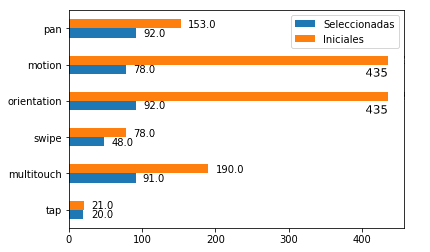
\includegraphics[width=0.8\textwidth]{imaxes/plots/selectedvsoriginal_features.png}
\caption{Características Iniciales VS Características Seleccionadas}
\label{fig:origianlvsselected}
\end{figure}


